\section{Limitations}
\label{sec:limitations}

The present work carries a number of limitations, organized here along four axes: epistemological, measurement, design, statistical. These are not retrospective hedges on the claims but an explicit boundary of what the data support and what they do not.

\subsection{Worldview as the primary source of the frame}
\label{subsec:worldview_first}

The DEIC program is built \emph{worldview-first}, and we take it as obligatory to name this order openly. The picture of how the architecture of empathy and non-empathy is organized crystallized for the authors before the data were collected --- out of psychoanalytic tradition, clinical observation, and the material of contemplative sources; the 131-item instrument was constructed specifically to test that picture. This is not an anti-pattern: most substantive theoretical syntheses in psychology (attachment theory in \citealp{bowlby1969}, mentalization theory in \citealp{fonagy2002}, the clinical tradition of psychopathy from \citealp{cleckley1941} to \citealp{hare1991}) are built in exactly the same way, and ``data first, theory second'' remains a rhetorical posture that rarely matches the actual process. We consider it more honest to name this order than to disguise it as the reverse.

Three specific risks follow from the worldview-first structure, and each requires explicit disclosure.

\paragraph{Confirmation risk.} The author of the frame has freedom in the choice of instrument, model specifications, aggregation methods, and interpretation, and may unconsciously optimize these decisions to confirm the initial intuition. The defense is pre-registered replication on an independent sample, collected and analyzed by a researcher not involved in the development of the frame and methodologically inclined to refute it. Without this step the present work must be read as an extended hypothesis, supported by one well-developed sample, rather than as an established fact.

\paragraph{LLM as a structural amplifier of the frame.} A substantial part of the work on refining constructs, formulating theoretical connections, and composing the final scaffolding was carried out in dialogue with large language models. This is methodologically significant not because of hallucinations (negligible in conceptual work) but because of the asymmetry of resistance. An LLM without its own biography, without a defensive structure, and without a source of skepticism outside the frame it is given is not a skeptical colleague but a logically coherent resonator: it extends the author's original frame into regions where a live interlocutor would stop and say ``wait''. The absence of friction here is not the absence of correction but active amplification. Partial compensation --- live disputation with a methodologically sober opponent not sharing the frame --- must be built into the preparation of wave 2 and explicitly recorded in methodology.

\paragraph{Three cardinal falsification conditions.} A frame is meaningful only if it pays a price. We formulate three cardinal conditions the failure of which destroys the corresponding parts of the program.

\emph{(a) Age-invariance of the CA$\to$ID$\to$\EAF{} channel in the 14--45 range.} If in an independent replication the parameters of the channel depend significantly on age within this range, the claim about a critical window of architectural formation closing before age 14 does not hold, and the entire architectural--ontogenetic interpretation of the program loses its ground.

\emph{(b) Orthogonality P$\perp$CA at the population level.} If in replication the correlation of P with CA is significantly positive, or the indirect effect CA$\to$P$\to$\EAF{} is significantly non-zero, the two-layer structure of P (architecture $+$ moral narrative, independent of childhood history) does not hold, and the model reverts to the standard clinical frame ``psychopathy as a consequence of trauma''.

\emph{(c) Reproducibility of the primary cluster (hi-P, lo-CA, lo-ID).} In the present data it was isolated by rule-based classification at $n = 144$ (10\% of the sample). If in an independent replication this cluster is not isolated or its size is radically smaller, the distinction between primary and secondary patterns returns to the status of a theoretical conjecture, and the claim of two etiological routes into the conditional architecture is not supported.

These three conditions are not a symbolic gesture but a real costly wager: the failure of any one of them will require a reformulation of the central part of the frame. Together with the three points of empirical resistance already observed in the present sample (§\ref{subsec:data_resistance_en}), they form the minimal set of tests that makes DEIC a falsifiable program rather than a self-confirming frame.

\subsection{Measurement limitations}

\paragraph{A as a formative, not reflective, construct.} This limitation is confirmed empirically in A-CFA Tier 5. On 17 carefully selected metacognitive items, CFI $= 0.866$, RMSEA $= 0.081$, $\omega$ by absolute loadings $= 0.947$, but the loadings are \emph{bipolar}---8 positive, 9 negative after external polarity alignment. When this latent A is substituted into conditional process SEM, the signs reverse relative to the theoretically weighted composite (A$_{\mathrm{lat}} \to$ ID $= +0.66$ against the composite's $-0.63$), and \IMM{} $= -0.00044$ [$-0.00267, +0.00052$] is nonsignificant. This is not a failure of analysis but empirical proof that the current item pool does not distinguish witnessing (observing-observation) from trauma hypervigilance (a pathological hypervigilance toward inner states). The main composite works because we built this distinction into the weights in advance. A dedicated A-scale is priority number one for wave 2.

\paragraph{M factor of low reliability.} $\omega = 0.546$ against $\omega > 0.89$ for the other five factors. Masking is weakly differentiated from P ($r_{\mathrm{latent}} = +0.82$). M-specific claims are not made in the paper; M is kept as a regulatory layer to be rebuilt in wave 2.

\paragraph{Post-hoc status of the ACE extension.} The extension of the ACE construct (treating ``don't remember / don't know'' as a positive signal of an adversity-relevant family or cognitive configuration rather than as missing data) is discussed substantively in §\ref{subsec:ace_extension} and validated on wave 1 through a full 6-factor oblique CFA re-fit (N~$=$~1468 against canonical 1426; CFI~$=$~0.960, RMSEA~$=$~0.062; bootstrap 95\,\% CIs of the indirect effects do not cross zero). Nevertheless this validation is \emph{post-hoc}: the recoding and re-fit were performed after the original publication CFA. A pre-registered wave 2 with an initially designed ACE-dissociation subscale and stated criteria in advance (McDonald's $\omega \ge 0.7$, $r(\text{ACE-dis}, \text{ID}_{\mathrm{lat}}) \ge 0.30$) is the condition for turning the extension from an observation into a claim about a reproducible structure. See §\ref{sec:future}.

\paragraph{Collapse of wave-1 scales into the present six-factor structure.} The progenitor instrument (DEIC-Inventory wave 1) had 12 content scales $+$ 2 controls (A, Lie). The published six-factor oblique CFA model is the result of two psychometrically forced collapse operations and one split operation.

\emph{Collapse of defenses (five into one, preserving the conceptual center).} Wave 1 had five scales of passive blocking: four mechanism-specific---suppression (\texttt{S}), dissociation (\texttt{D}), affective isolation (\texttt{AIS}), affective flatness (\texttt{F})---and one experientially central, the \emph{Internal Dissonance Scale} (\texttt{IDS}), measuring the subjective experience ``an empathic response began but does not continue; I want to feel but I cannot.'' The choice of a single ID latent in the main model is a decision of \emph{parsimony}, not a verdict on the structure: on our data the five-factor oblique CFA converges (CFI~$=$~0.891, RMSEA~$=$~0.077), but the latent correlations among the five defenses have $|r|$ in the range $0.66$--$0.89$ with partially opposite signs (a structure of mixed signs characteristic of semi-collapsed collinearity). At this level of separability the five separate latents do not yield a clinically or statistically stable distinction; meanwhile, a common ID latent absorbs most of the variation. Wave 2 (the present work) preserves the conceptual center unchanged and simply removes ``Scale'' from the label: \texttt{IDS} $\to$ \textbf{ID} (\emph{Internal Dissonance}). The extension consists in the fact that the four mechanism-specific scales (S, D, AIS, F) are absorbed into the same latent as surface manifestations of a single field. Substantively this agrees with Fonagy (the absence of a mentalizing field as a condition, not a sum of mechanisms) and with Di Giuseppe \& Perry \citep{digiuseppe2024} (defenses as an integrated network rather than parallel traits).

\emph{Limitation of parsimony.} Absorption is not equivalent to proof of unidimensionality. In an additional bifactor analysis (§\ref{subsec:id_bifactor}), a general factor model (ID\textsubscript{g} plus five uncorrelated specific factors) exceeds the unifactor ID model on the principal indices and shows that the general ID explains about 57\,\% of the total variance (ECV\textsubscript{global}~$=$~0.57), with notable per-subscale heterogeneity: FLA and IDS are almost fully absorbed by the general ID (ECV~$=$~0.86 and 0.66 respectively), DIS and AIS retain about half of their unique variance (ECV~$\approx$~0.54, 0.53), while SUP remains to a significant degree a separate construct (ECV~$=$~0.31). Clinically this means: suppression (SUP) is the worst-absorbed by the umbrella latent, and in wave 2 should with high probability be restored as a separate latent; FLA, on the contrary, is well described by the general ID and can remain a reliable indicator of it; DIS and AIS stand in between---they require either additional items for clean separation or a bifactor level in the published model. The phenomenological distinctions among surface mechanisms---suppression (ego-syntonic, conscious), dissociation (ego-dystonic, automatic), affective isolation (content present, feeling severed), flatness (affective signal absent)---are hidden in the published unifactor ID model; in the bifactor model and in the wave-2 design they are restored.

\emph{Collapse of the contextual layer (ACE $+$ CA $\to$ CA).} Wave 1 distinguished a general index of adverse childhood experiences (\texttt{ACE} in the spirit of Felitti et al.) and a narrow scale of childhood adversity (\texttt{CA}, with an emphasis on early-years relational trauma). In our sample these turned out to be interchangeable indicators of one latent ($r > 0.8$), so the published model uses a single \textbf{CA} as the latent of early relational-stress history. The wave-1 distinction among types of trauma (domestic violence, emotional deprivation, attachment instability) is hidden in this aggregation. Additional wave-1 contextual scales---emotional context (\texttt{EC}) and an affective-dissociative indicator (\texttt{ADI})---are retained as observed composites for descriptive use but do not enter the main CFA as latents.

\emph{Split of empathy (one into two).} The opposite operation: the wave-1 general empathy scale \texttt{E} was split into \EAF{} and \Ecog{} post-hoc, in response to the P$\leftrightarrow$E paradox in the original model and in agreement with the multidimensional tradition of Davis \citep{davis1983}. This is an acquisition, not a loss; but it is post-hoc and must be reproduced on pre-registered items separated by design (see below---statistical limitations).

\begin{figure}[htbp]
\centering
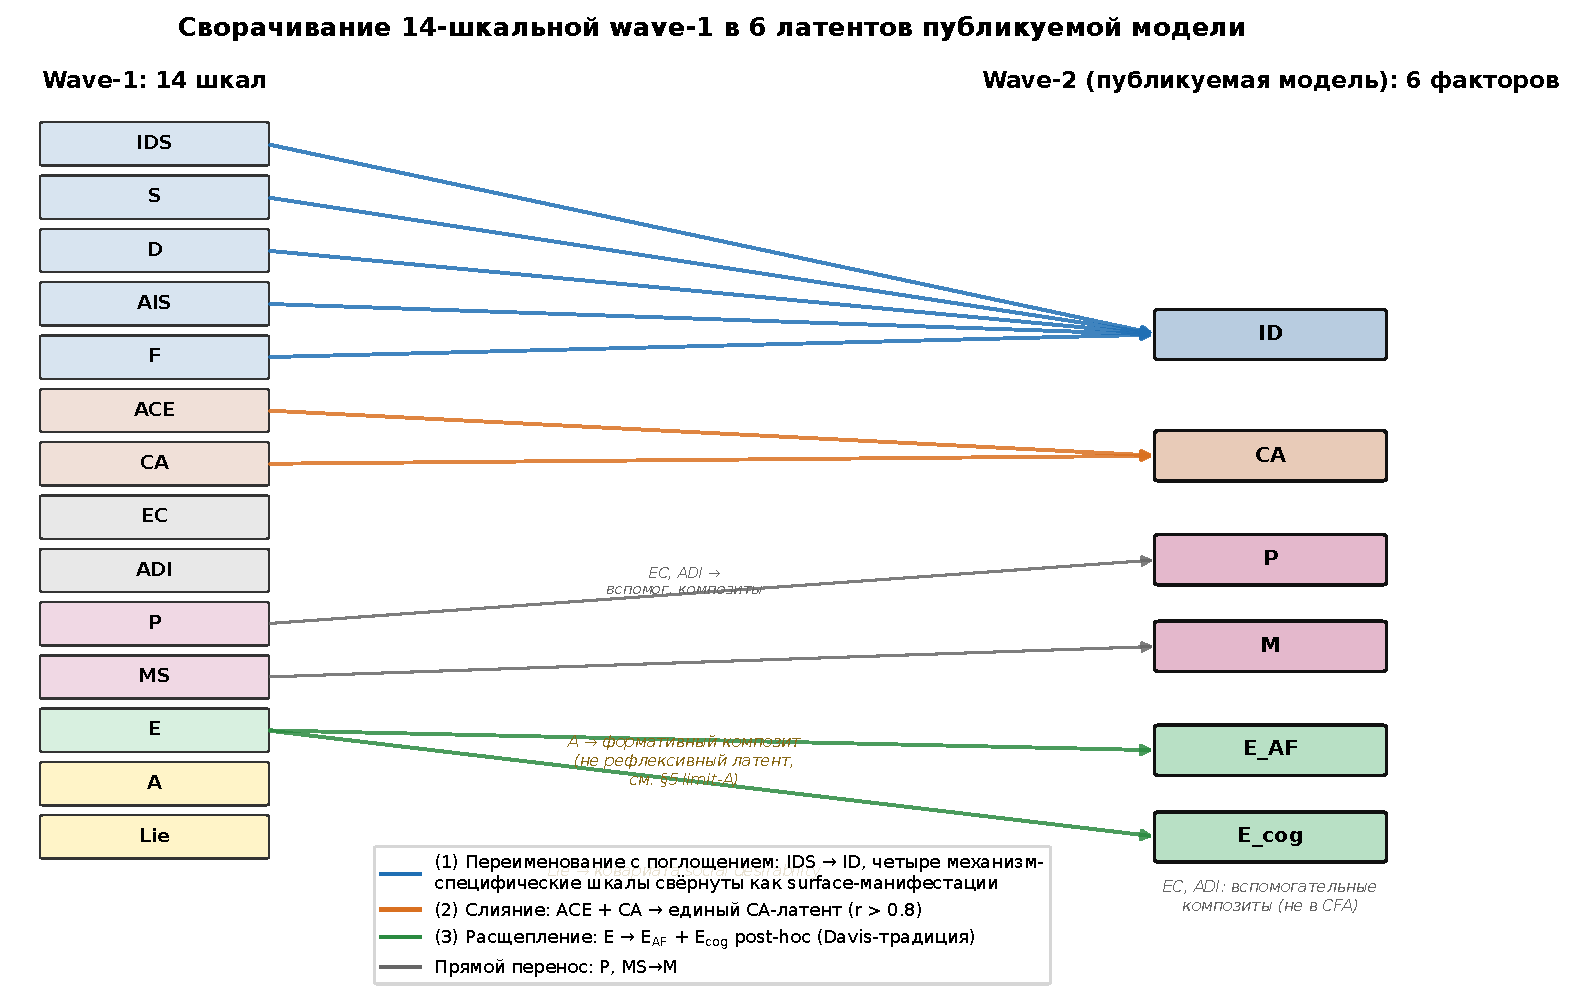
\includegraphics[width=0.95\linewidth]{figures/fig9_wave_mapping.pdf}
\caption[Wave-1 to wave-2 transition map]{Map of the transition from 14 wave-1 scales to 6 latents of the published model. Blue arrows: renaming with absorption (IDS $\to$ ID, together with S, D, AIS, F as surface manifestations of one field); orange: merger of two indicators of early history (ACE + CA $\to$ CA); green: split of the general empathy scale (E $\to$ \EAF{} + \Ecog{}); gray: passthrough (P, MS $\to$ M). EC, ADI retained as auxiliary observed composites; A, Lie---control scales.}
\label{fig:wave_mapping}
\end{figure}

\emph{Resulting map.} 12 wave-1 content scales $\to$ 6 latents of the published model: \texttt{IDS} $\to$ \textbf{ID} (renaming with absorption of \{\texttt{S, D, AIS, F}\} as inseparable surface manifestations of the same field); \{\texttt{ACE, CA}\} $\to$ CA (merger of two indicators of early relational history into a single latent); \texttt{P} $\to$ P; \texttt{MS} $\to$ M; \texttt{E} $\to$ \{\EAF, \Ecog\} (post-hoc split, the only expansion operation); \{\texttt{EC, ADI}\} $\to$ auxiliary observed composites. A is separated as a formative composite; Lie is a social-desirability covariate correcting E and ID in the applied integral metrics. The published six-factor structure is the minimal one the data support. The phenomenological and typological distinctions hidden by that minimality are a task for wave 2.

\paragraph{Multi-scale weights in \texttt{questions.json}---an innovation and its scoring artifact.} The explicit a priori assignment to each item of a vector of weights across several factors is a substantive innovation of the instrument, not a methodological carelessness: most empathy questionnaires pretend that simple structure holds and assign an item to a single scale, losing the share of variance that sits at the intersections of constructs. DEIC brings this cross-structural aspect out of implicit statistical artifact and into an explicit theoretical declaration that can be criticized and validated (its closest psychometric relative is the a priori bifactor model). However, composite sum-scoring with multi-scale weights algebraically inflates correlations among composites: an item with nonzero weights in two composites is counted on both sides of the equation when those composites correlate. In our sample the average inflation is $\sim 0.18$, with a maximum of $0.68$ with a sign change for P$\leftrightarrow$E. Latent factor scores are immune to this problem because CFA correctly partitions common and specific variance. The wave-2 solution is not the abandonment of the innovation but its separation into two independent layers in \texttt{questions.json}: \texttt{factor\_weights} (a vector for CFA with explicitly prescribed cross-loadings---the theoretical layer remains) and \texttt{primary\_scale} (the single factor for composite sum-scoring---one item, one composite). Composites are published as orienting without algebraic inflation; latent scores as the main scientific result. The innovation is retained in full and becomes two-layered by construction.

\paragraph{Self-report only.} No informant report, no behavioral measures, no physiological convergent measures. Especially critical for A, where self-report has a circular-validity limitation (an accurate report on attention requires attention).

\paragraph{The secondary psychopathic subgroup is small.} $n = 65$. Rule-based $2 \times 2$ yields a stable direction, but effect sizes in the secondary cell have wide CIs and require a clinical sample for confirmation.

\subsection{Design-related limitations}

\paragraph{Cross-sectional.} No temporal axis, no pre/post therapy design, no retest stability. Consequence: it is impossible to distinguish stable A from transient A, impossible to test the longitudinal predictions formulated in §\ref{subsec:falsifiers}, and impossible to distinguish empirically the direction of causation in the CA--ID pair (assumed theoretically but statistically unidentified).

\paragraph{Monolingual sample.} Russian-language internet recruitment; a self-selected sample. Cultural, linguistic, and platform biases are present. Cross-cultural validation (EN, ES, CH, AR) with invariance testing is the obligatory next step.

\paragraph{Age skew} toward 18--37; the 38$+$ subsample ($n = 50$) is small. Suppressor mediation is stable at 18--37 and weakens at 38$+$; the mechanism is unclear---post-therapy effects, survivor bias, developmental shift---and requires an age-stratified sample.

\paragraph{Self-selection through Telegram/VK.} The survey requires an introductory metacognitive vocabulary; possibly this form of selection already shifts the A distribution to the right relative to the general population. The data do not support generalization to non-reflective subpopulations.

\paragraph{The ``befriends-psychopaths'' subsample and individual-level ethics.}
\label{subsec:limitations_befriends}
The archetype of the empathic counterpart in a dyad with a psychopath (hi-E $+$ hi-P in the $+++-$ octant) is empirically confirmed but represented in the sample by only $n = 3$ respondents ($0.19\,\%$). None of them endorsed any free-text diagnostic category; self-descriptions of this profile in the open field are absent: the archetype is systematically invisible to self-report. Retrospective power estimate: detection of $d = 0.5$ in this subgroup requires $n \approx 150$; $d = 1.0$---$n \approx 30$. In the present wave the profile is recorded descriptively, without parametric comparisons. Wave 2 requires targeted sampling of this configuration. \emph{Ethical limitation:} one of the three respondents is known to us biographically; therefore any individual-level characteristics of this subgroup are published only as aggregated centroids ($n = 3$), and individual-level data from the paper is excluded and not released to the open supplementary.

\subsection{Statistical limitations}

\paragraph{Multivariate non-normality of the data and robust fit indices.} Mardia $p < 0.0001$. Two approximate robust recomputations are implemented. \textbf{(a)}~Bootstrap approximation of Satorra--Bentler scaling (in \texttt{tier4\_analyses.py}). \textbf{(b)}~Satorra--Bentler T$_1$ via \texttt{semopy.stats.calc\_chi2\_sb} with a fourth-moment weight matrix from \texttt{prepare\_wls} over the ML fit: $\chi^2_{\mathrm{SB}}(120) = 934.25$, CFI$_{\mathrm{SB}} = 0.873$, RMSEA$_{\mathrm{SB}} = 0.098$, scaling factor $c = 0.552$. The atypical $c < 1$ (the ML-$\chi^2$ is deflated relative to the SB-corrected) and the drop of CFI from $0.950$ to $0.873$ are two independent signals that the substantive conclusions of the paper should be evaluated on latent factor scores (robust to this correction) rather than on global fit indices. Exact MLR SEs and WLSMV on raw ordinal items require \texttt{lavaan} in R for final publication; this is an infrastructural gap, not a substantive one, and the reviewer standard requires it explicitly.

\paragraph{Conditional process SEM on the composite A moderator.} After A-CFA, the correct implementation is a transition to structural modeling of A as a latent, accounting for its bipolar nature. In the current form, A moderation rests on a theoretically weighted composite; this works but requires duplication in structural form.

\paragraph{Post-hoc character of the factor separation \EAF{}/\Ecog{}.} The separation of cognitive and affective empathy was established post-hoc in response to the P$\leftrightarrow$E paradox in the original model. Pre-registered replication on items separated by design is a necessary condition for the stability of this distinction.

\subsection{Theoretical gaps}

These are not limitations of the present paper in the strict sense but \emph{missing elements in the theory} that the program is to build. We list them explicitly because the boundary of the known is part of empirical work.

\paragraph{Temporal framework.} The theory in its current form is a cross-sectional snapshot. All its substantive vocabulary (``automatism,'' ``awareness'') is temporal. A three-timescale framework is required: fast (ms--s, stimulus $\to$ activation of ID $\to$ suppression of \EAF{}); meso (weeks--months, repeated A activations in therapy $\to$ gradual decoupling); slow (years--decades, ACE $\to$ formation of ID pattern $\to$ recruitment of P or not). A separate paper ``\DEIC{} dynamics: temporal architecture of empathy blocking'' is planned.

\paragraph{The ID $\leftrightarrow$ P switch mechanism.} ID and P are empirically separable. But \emph{what decides} in a concrete context which mechanism is recruited---the theory does not say. Three candidate frames: cost/benefit (P---when suppression of empathy is advantageous; ID---when feeling is intolerable); predictive coding (ID---a bottom-up overload signal; P---a top-down model signal); conflict monitoring (ID blocks feeling; P blocks action). The working choice is predictive coding; exposition in a separate paper.

\paragraph{The mechanism of A's therapeutic power.} A empirically moderates both paths. The mechanism is undetermined. Candidates: A increases the temporal resolution of self-observation, catching a defense before it completes; A decomposes the automatic binding ID$\leftrightarrow$\EAF{}-suppression; A $=$ metacognitive working memory with limited capacity. Exposition in a separate paper.

\paragraph{Individual differences in A-trainability.} The instrument measures current A but there is no model of what \emph{permits} A to be trained. Candidates: working memory capacity, interoceptive accuracy, language-mediation capacity, safety-context stability. Clinical significance: prediction of who will respond to A-based therapy.

\paragraph{Developmental branching in $2\times 2$.} Primary, secondary, traumatic, and baseline are described topologically. The route by which a child ends up in each cell is a separate theoretical task. The Karpman hypothesis (primary constitutional, secondary acquired) is testable with early CA/temperament markers on a longitudinal child sample.

\paragraph{Evolutionary-ecological substrate.} Why is empathy default-on? Why two separable mechanisms of switching-off? Why is P stable in the population as an ESS at low frequency? \DEIC{} is not connected to the evolutionary literature; that is the burden of the theory-of-everything direction and explicitly falls outside the present paper.

\paragraph{Observer reflexivity.} The observer's A is a condition of seeing A in the observed. In therapy this is an operational reality (a therapist with low A does not see the ID activations of the patient). In research, the measurement apparatus contains the measured quantity. An analogy with the observer problem in quantum mechanics is not mystical but structural. It deserves a separate methodological section in a programmatic paper.
